% Created by tikzDevice version 0.11 on 2019-01-25 13:45:32
% !TEX encoding = UTF-8 Unicode
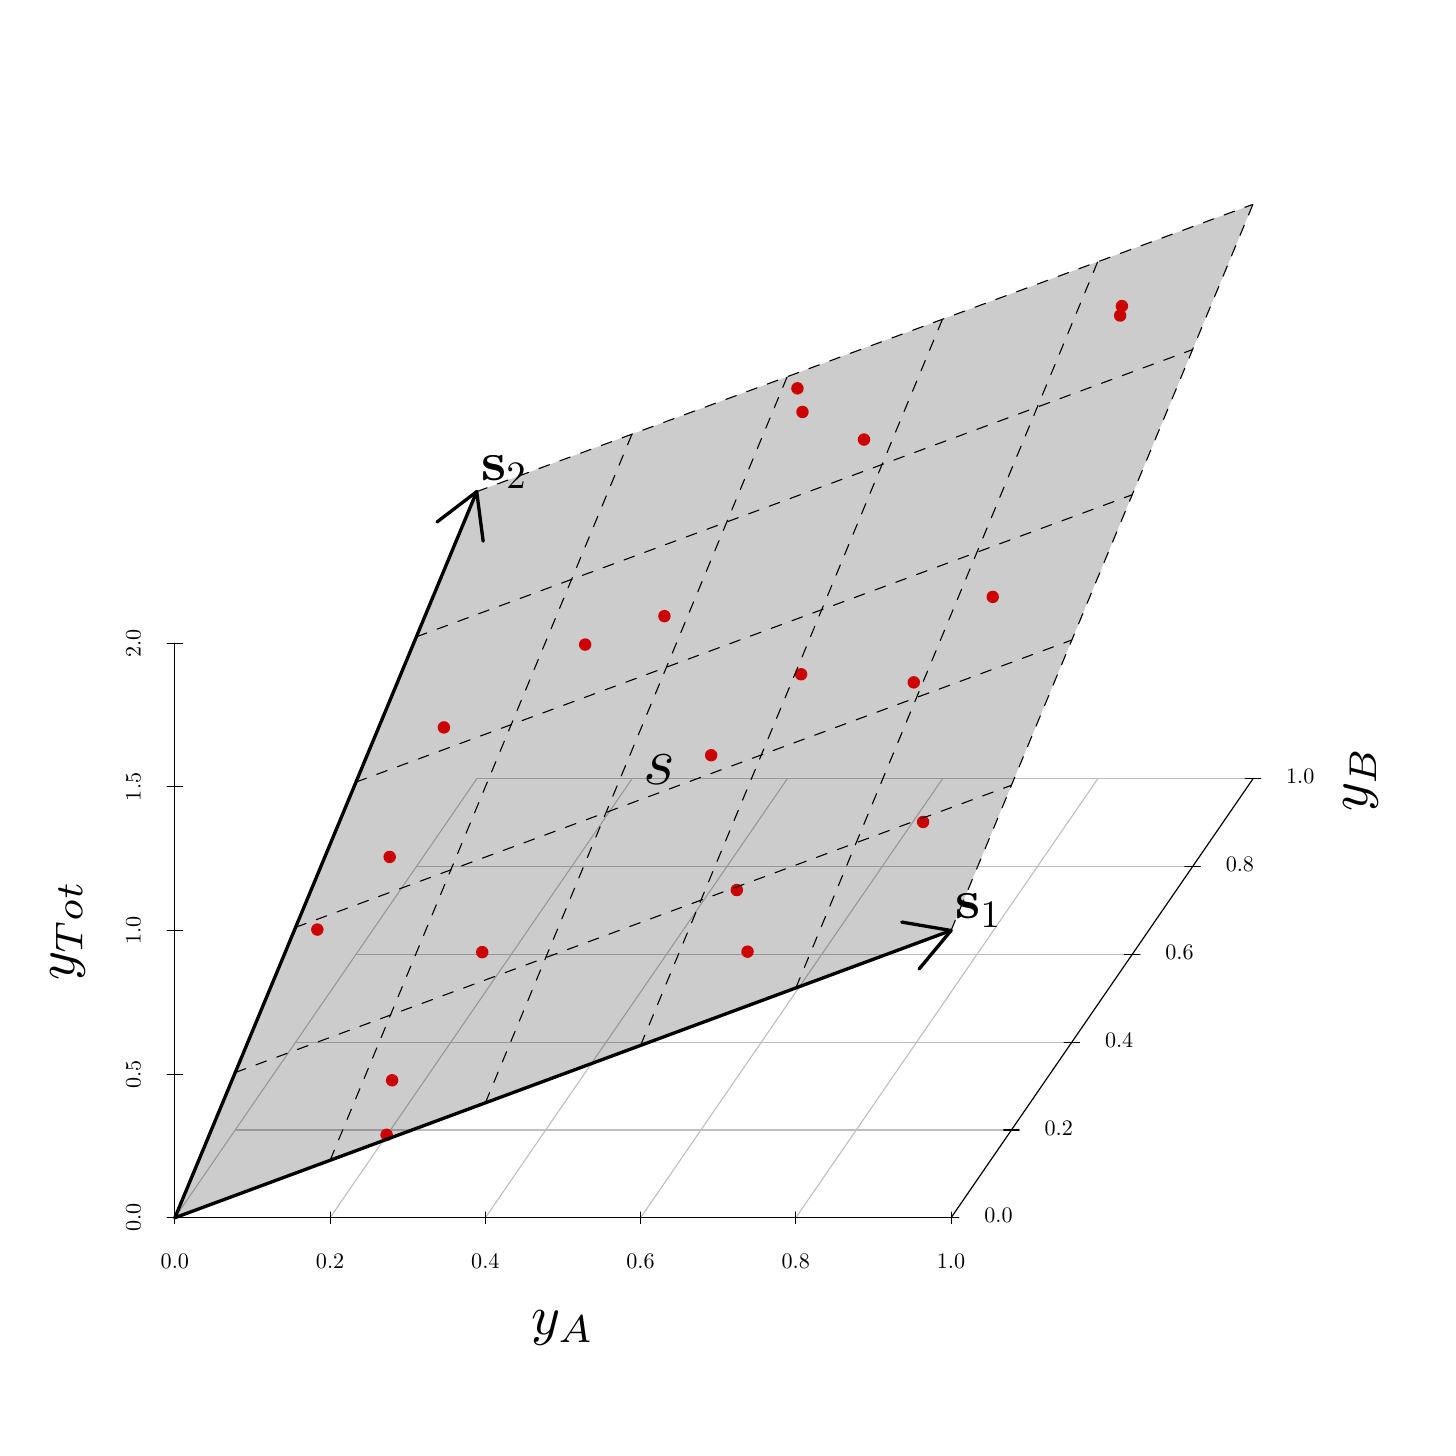
\begin{tikzpicture}[x=1pt,y=1pt]
\definecolor{fillColor}{RGB}{255,255,255}
\path[use as bounding box,fill=fillColor,fill opacity=0.00] (0,0) rectangle (505.89,505.89);
\begin{scope}
\path[clip] ( 37.20, 61.20) rectangle (468.69,456.69);
\definecolor{drawColor}{RGB}{190,190,190}

\path[draw=drawColor,line width= 0.4pt,line join=round,line cap=round] ( 53.18, 75.85) -- (162.26,234.44);

\path[draw=drawColor,line width= 0.4pt,line join=round,line cap=round] (109.28, 75.85) -- (218.36,234.44);

\path[draw=drawColor,line width= 0.4pt,line join=round,line cap=round] (165.38, 75.85) -- (274.45,234.44);

\path[draw=drawColor,line width= 0.4pt,line join=round,line cap=round] (221.47, 75.85) -- (330.55,234.44);

\path[draw=drawColor,line width= 0.4pt,line join=round,line cap=round] (277.57, 75.85) -- (386.65,234.44);

\path[draw=drawColor,line width= 0.4pt,line join=round,line cap=round] (333.67, 75.85) -- (442.74,234.44);

\path[draw=drawColor,line width= 0.4pt,line join=round,line cap=round] ( 53.18, 75.85) -- (333.67, 75.85);

\path[draw=drawColor,line width= 0.4pt,line join=round,line cap=round] ( 75.00,107.57) -- (355.48,107.57);

\path[draw=drawColor,line width= 0.4pt,line join=round,line cap=round] ( 96.81,139.28) -- (377.30,139.28);

\path[draw=drawColor,line width= 0.4pt,line join=round,line cap=round] (118.63,171.00) -- (399.11,171.00);

\path[draw=drawColor,line width= 0.4pt,line join=round,line cap=round] (140.44,202.72) -- (420.93,202.72);

\path[draw=drawColor,line width= 0.4pt,line join=round,line cap=round] (162.26,234.44) -- (442.74,234.44);
\definecolor{drawColor}{RGB}{0,0,0}

\path[draw=drawColor,line width= 0.4pt,line join=round,line cap=round] (330.86, 75.85) -- (336.47, 75.85);

\path[draw=drawColor,line width= 0.4pt,line join=round,line cap=round] (352.68,107.57) -- (358.29,107.57);

\path[draw=drawColor,line width= 0.4pt,line join=round,line cap=round] (374.49,139.28) -- (380.10,139.28);

\path[draw=drawColor,line width= 0.4pt,line join=round,line cap=round] (396.31,171.00) -- (401.92,171.00);

\path[draw=drawColor,line width= 0.4pt,line join=round,line cap=round] (418.12,202.72) -- (423.73,202.72);

\path[draw=drawColor,line width= 0.4pt,line join=round,line cap=round] (439.94,234.44) -- (445.55,234.44);

\path[draw=drawColor,line width= 0.4pt,line join=round,line cap=round] ( 53.18, 73.77) -- ( 53.18, 77.92);

\path[draw=drawColor,line width= 0.4pt,line join=round,line cap=round] (109.28, 73.77) -- (109.28, 77.92);

\path[draw=drawColor,line width= 0.4pt,line join=round,line cap=round] (165.38, 73.77) -- (165.38, 77.92);

\path[draw=drawColor,line width= 0.4pt,line join=round,line cap=round] (221.47, 73.77) -- (221.47, 77.92);

\path[draw=drawColor,line width= 0.4pt,line join=round,line cap=round] (277.57, 73.77) -- (277.57, 77.92);

\path[draw=drawColor,line width= 0.4pt,line join=round,line cap=round] (333.67, 73.77) -- (333.67, 77.92);

\path[draw=drawColor,line width= 0.4pt,line join=round,line cap=round] ( 50.38, 75.85) -- ( 55.99, 75.85);

\path[draw=drawColor,line width= 0.4pt,line join=round,line cap=round] ( 50.38,127.75) -- ( 55.99,127.75);

\path[draw=drawColor,line width= 0.4pt,line join=round,line cap=round] ( 50.38,179.65) -- ( 55.99,179.65);

\path[draw=drawColor,line width= 0.4pt,line join=round,line cap=round] ( 50.38,231.55) -- ( 55.99,231.55);

\path[draw=drawColor,line width= 0.4pt,line join=round,line cap=round] ( 50.38,283.45) -- ( 55.99,283.45);
\end{scope}
\begin{scope}
\path[clip] (  0.00,  0.00) rectangle (505.89,505.89);
\definecolor{drawColor}{RGB}{0,0,0}

\node[text=drawColor,anchor=base,inner sep=0pt, outer sep=0pt, scale=  0.80] at ( 53.18, 57.60) {0.0};

\node[text=drawColor,anchor=base,inner sep=0pt, outer sep=0pt, scale=  0.80] at (109.28, 57.60) {0.2};

\node[text=drawColor,anchor=base,inner sep=0pt, outer sep=0pt, scale=  0.80] at (165.38, 57.60) {0.4};

\node[text=drawColor,anchor=base,inner sep=0pt, outer sep=0pt, scale=  0.80] at (221.47, 57.60) {0.6};

\node[text=drawColor,anchor=base,inner sep=0pt, outer sep=0pt, scale=  0.80] at (277.57, 57.60) {0.8};

\node[text=drawColor,anchor=base,inner sep=0pt, outer sep=0pt, scale=  0.80] at (333.67, 57.60) {1.0};

\node[text=drawColor,rotate= 90.00,anchor=base,inner sep=0pt, outer sep=0pt, scale=  0.80] at ( 40.80, 75.85) {0.0};

\node[text=drawColor,rotate= 90.00,anchor=base,inner sep=0pt, outer sep=0pt, scale=  0.80] at ( 40.80,127.75) {0.5};

\node[text=drawColor,rotate= 90.00,anchor=base,inner sep=0pt, outer sep=0pt, scale=  0.80] at ( 40.80,179.65) {1.0};

\node[text=drawColor,rotate= 90.00,anchor=base,inner sep=0pt, outer sep=0pt, scale=  0.80] at ( 40.80,231.55) {1.5};

\node[text=drawColor,rotate= 90.00,anchor=base,inner sep=0pt, outer sep=0pt, scale=  0.80] at ( 40.80,283.45) {2.0};
\end{scope}
\begin{scope}
\path[clip] ( 37.20, 61.20) rectangle (468.69,456.69);
\definecolor{drawColor}{RGB}{0,0,0}

\node[text=drawColor,anchor=base west,inner sep=0pt, outer sep=0pt, scale=  0.80] at (345.67, 74.01) {0.0};

\node[text=drawColor,anchor=base west,inner sep=0pt, outer sep=0pt, scale=  0.80] at (367.48,105.73) {0.2};

\node[text=drawColor,anchor=base west,inner sep=0pt, outer sep=0pt, scale=  0.80] at (389.30,137.45) {0.4};

\node[text=drawColor,anchor=base west,inner sep=0pt, outer sep=0pt, scale=  0.80] at (411.11,169.16) {0.6};

\node[text=drawColor,anchor=base west,inner sep=0pt, outer sep=0pt, scale=  0.80] at (432.93,200.88) {0.8};

\node[text=drawColor,anchor=base west,inner sep=0pt, outer sep=0pt, scale=  0.80] at (454.74,232.60) {1.0};

\path[draw=drawColor,line width= 0.4pt,line join=round,line cap=round] ( 53.18, 75.85) --
	(333.67, 75.85);
\end{scope}
\begin{scope}
\path[clip] (  0.00,  0.00) rectangle (505.89,505.89);
\definecolor{drawColor}{RGB}{0,0,0}

\node[text=drawColor,anchor=base,inner sep=0pt, outer sep=0pt, scale=  2.00] at (193.42, 33.60) {$y_A$};
\end{scope}
\begin{scope}
\path[clip] ( 37.20, 61.20) rectangle (468.69,456.69);
\definecolor{drawColor}{RGB}{0,0,0}

\path[draw=drawColor,line width= 0.4pt,line join=round,line cap=round] (333.67, 75.85) --
	(442.74,234.44);
\end{scope}
\begin{scope}
\path[clip] (  0.00,  0.00) rectangle (505.89,505.89);
\definecolor{drawColor}{RGB}{0,0,0}

\node[text=drawColor,rotate= 90.00,anchor=base,inner sep=0pt, outer sep=0pt, scale=  2.00] at (484.29,234.44) {$y_B$};
\end{scope}
\begin{scope}
\path[clip] ( 37.20, 61.20) rectangle (468.69,456.69);
\definecolor{drawColor}{RGB}{0,0,0}

\path[draw=drawColor,line width= 0.4pt,line join=round,line cap=round] ( 53.18, 75.85) --
	( 53.18,283.45);
\end{scope}
\begin{scope}
\path[clip] (  0.00,  0.00) rectangle (505.89,505.89);
\definecolor{drawColor}{RGB}{0,0,0}

\node[text=drawColor,rotate= 90.00,anchor=base,inner sep=0pt, outer sep=0pt, scale=  2.00] at ( 16.80,179.65) {$y_{Tot}$};
\end{scope}
\begin{scope}
\path[clip] ( 37.20, 61.20) rectangle (468.69,456.69);
\definecolor{fillColor}{RGB}{255,0,0}

\path[fill=fillColor] (278.15,375.56) circle (  2.25);

\path[fill=fillColor] (279.97,367.03) circle (  2.25);

\path[fill=fillColor] (395.40,405.29) circle (  2.25);

\path[fill=fillColor] (394.76,401.87) circle (  2.25);

\path[fill=fillColor] (302.20,357.05) circle (  2.25);

\path[fill=fillColor] (201.44,282.97) circle (  2.25);

\path[fill=fillColor] (230.08,293.24) circle (  2.25);

\path[fill=fillColor] (150.40,253.03) circle (  2.25);

\path[fill=fillColor] (348.72,300.19) circle (  2.25);

\path[fill=fillColor] (279.47,272.24) circle (  2.25);

\path[fill=fillColor] (130.81,206.23) circle (  2.25);

\path[fill=fillColor] (246.98,242.98) circle (  2.25);

\path[fill=fillColor] (320.19,269.31) circle (  2.25);

\path[fill=fillColor] (104.67,179.99) circle (  2.25);

\path[fill=fillColor] (164.26,171.82) circle (  2.25);

\path[fill=fillColor] (256.24,194.27) circle (  2.25);

\path[fill=fillColor] (323.55,218.87) circle (  2.25);

\path[fill=fillColor] (131.69,125.53) circle (  2.25);

\path[fill=fillColor] (260.12,172.00) circle (  2.25);

\path[fill=fillColor] (129.70,105.84) circle (  2.25);
\definecolor{fillColor}{RGB}{0,0,0}

\path[fill=fillColor,fill opacity=0.20] ( 53.18, 75.85) --
	(162.26,338.24) --
	(442.74,442.04) --
	(333.67,179.65) --
	cycle;
\definecolor{drawColor}{RGB}{0,0,0}

\path[draw=drawColor,line width= 0.4pt,dash pattern=on 4pt off 4pt ,line join=round,line cap=round] ( 53.18, 75.85) -- (162.26,338.24);

\path[draw=drawColor,line width= 0.4pt,dash pattern=on 4pt off 4pt ,line join=round,line cap=round] (109.28, 96.61) -- (218.36,359.00);

\path[draw=drawColor,line width= 0.4pt,dash pattern=on 4pt off 4pt ,line join=round,line cap=round] (165.38,117.37) -- (274.45,379.76);

\path[draw=drawColor,line width= 0.4pt,dash pattern=on 4pt off 4pt ,line join=round,line cap=round] (221.47,138.13) -- (330.55,400.52);

\path[draw=drawColor,line width= 0.4pt,dash pattern=on 4pt off 4pt ,line join=round,line cap=round] (277.57,158.89) -- (386.65,421.28);

\path[draw=drawColor,line width= 0.4pt,dash pattern=on 4pt off 4pt ,line join=round,line cap=round] (333.67,179.65) -- (442.74,442.04);

\path[draw=drawColor,line width= 0.4pt,dash pattern=on 4pt off 4pt ,line join=round,line cap=round] ( 53.18, 75.85) -- (333.67,179.65);

\path[draw=drawColor,line width= 0.4pt,dash pattern=on 4pt off 4pt ,line join=round,line cap=round] ( 75.00,128.33) -- (355.48,232.13);

\path[draw=drawColor,line width= 0.4pt,dash pattern=on 4pt off 4pt ,line join=round,line cap=round] ( 96.81,180.80) -- (377.30,284.61);

\path[draw=drawColor,line width= 0.4pt,dash pattern=on 4pt off 4pt ,line join=round,line cap=round] (118.63,233.28) -- (399.11,337.09);

\path[draw=drawColor,line width= 0.4pt,dash pattern=on 4pt off 4pt ,line join=round,line cap=round] (140.44,285.76) -- (420.93,389.56);

\path[draw=drawColor,line width= 0.4pt,dash pattern=on 4pt off 4pt ,line join=round,line cap=round] (162.26,338.24) -- (442.74,442.04);

\path[draw=drawColor,line width= 1.2pt,line join=round,line cap=round] ( 53.18, 75.85) -- (333.67,179.65);

\path[draw=drawColor,line width= 1.2pt,line join=round,line cap=round] (322.13,165.75) --
	(333.67,179.65) --
	(315.86,182.69);

\path[draw=drawColor,line width= 1.2pt,line join=round,line cap=round] ( 53.18, 75.85) -- (162.26,338.24);

\path[draw=drawColor,line width= 1.2pt,line join=round,line cap=round] (164.59,320.32) --
	(162.26,338.24) --
	(147.91,327.26);

\node[text=drawColor,anchor=base west,inner sep=0pt, outer sep=0pt, scale=  2.00] at (335.27,183.85) {\bfseries s};

\node[text=drawColor,anchor=base west,inner sep=0pt, outer sep=0pt, scale=  1.40] at (344.34,180.84) {1};

\node[text=drawColor,anchor=base west,inner sep=0pt, outer sep=0pt, scale=  2.00] at (163.87,342.44) {\bfseries s};

\node[text=drawColor,anchor=base west,inner sep=0pt, outer sep=0pt, scale=  1.40] at (172.94,339.43) {2};

\node[text=drawColor,anchor=base west,inner sep=0pt, outer sep=0pt, scale=  1.00] at (222.57,232.24) {{\Huge $\mathfrak{s}$}};
\end{scope}
\end{tikzpicture}
